\documentclass{standalone}
% 
% \pgfmathdeclarefunction{gauss}{2}{%
%   \pgfmathparse{1/(#2*sqrt(2*pi))*exp(-((x-#1)^2)/(2*#2^2))}%
% }
\usepackage{tkz-euclide}
\usetkzobj{all}
\renewcommand{\familydefault}{\sfdefault}
\usepackage{calc,tikz}
\usetikzlibrary{calc}
\usepackage{pgfplots}
\usetikzlibrary{patterns}
\begin{document}
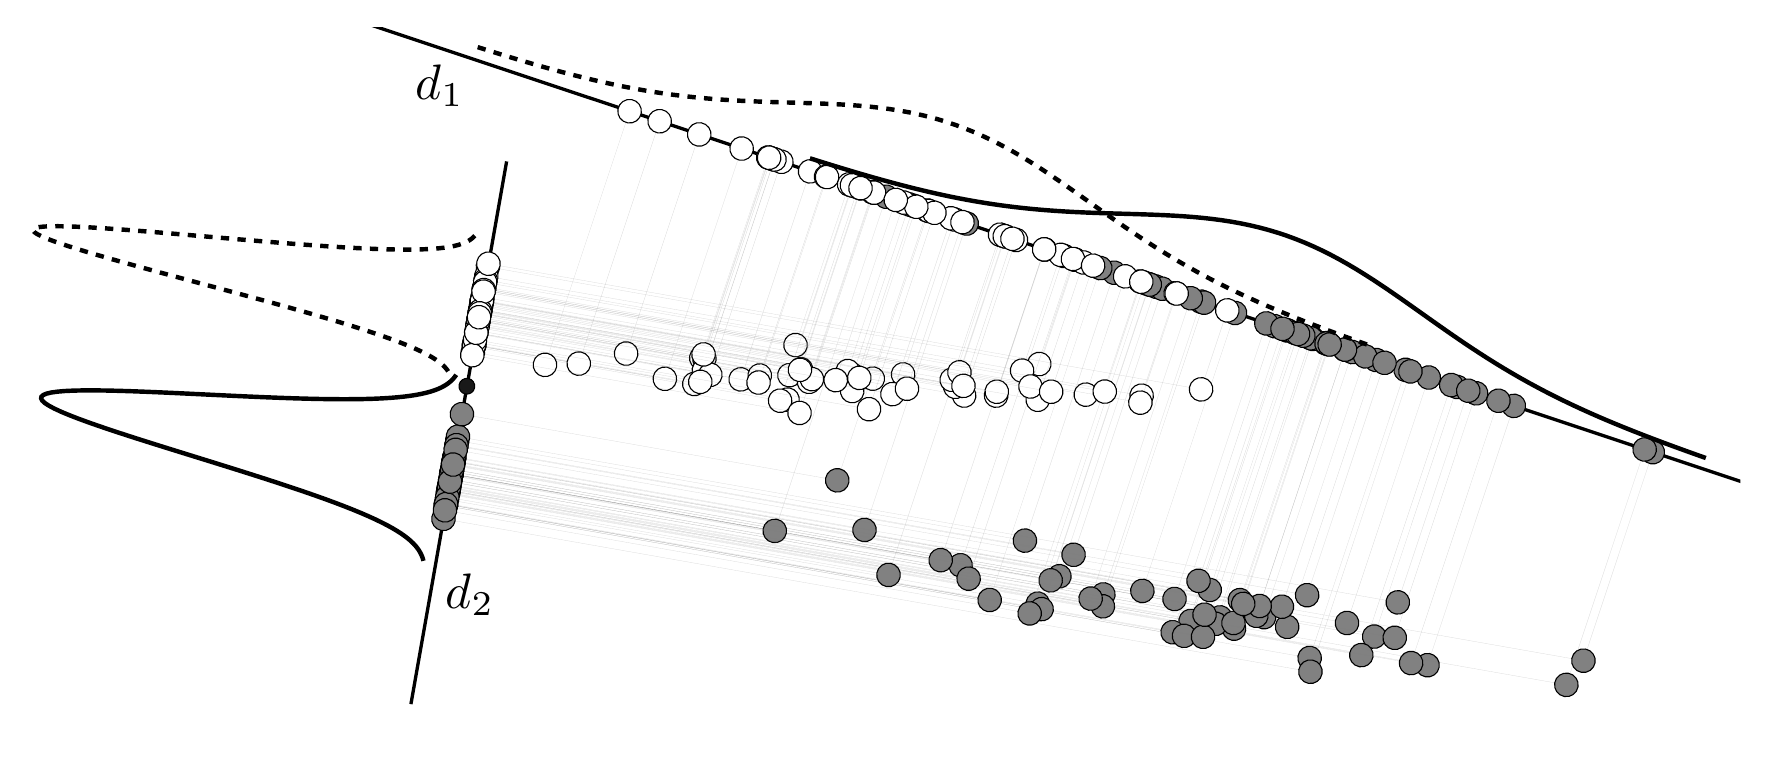
\begin{tikzpicture}[>=stealth]
    \clip (-14.25, -1.8) rectangle (7.5, 7.2);
    \def\normaltwo{\x,{4*1/exp(((\x-0)^2)/2)}}
    % \node [scale = 2] at (6.5, 3.3) {PCA procedure};
    %%%%%%%%% block 1%%%%%%%%%%%%%%%%%
    \begin{scope}[rotate = -10]
    \tkzDefPoint(-15, 6){A}
    \tkzDefPoint(12, 2){B}
    \tkzDefPoint(-9, 4){C}
    \tkzDefPoint(-9, -3){D}
    \draw [ very thick] (A) -- (B);
    \draw [ very thick] (C) -- (D);


    \begin{scope}
        % \draw [rounded corners = 2pt, thick] (-2.7, -3.2) rectangle (3.3, 2.75);
        \begin{scope}[rotate = 0, yshift = 0cm]
            \foreach \x/\y/\z in {0.57/-0.24/0, 2.14/-0.44/1, 2.9/-0.03/2, -1.38/-0.36/3, 1.14/0.13/4, 1.48/-0.03/5, -1.17/0.03/6, -2.43/-0.05/7, -1.68/0.4/8, 0.93/-0.13/9, -1.04/0.33/10, -1.27/-0.04/11, 1.13/-0.24/12, 2.53/0.08/13, 3.16/0.0/14, 5.57/0.13/15, 0.37/-0.42/16, 0.52/-0.44/17, -0.58/-0.1/18, 1.79/-0.1/19, -0.56/-0.25/20, -0.73/-0.18/21, 3.63/-0.27/22, -2.3/-0.2/23, 2.18/-0.61/24, 2.78/-0.29/25, -1.99/-0.42/26, 0.89/-0.22/27, 0.32/0.0/28, -4.83/-0.03/29, 0.76/-0.41/30, -2.69/-0.03/31, 3.12/0.45/32, 3.42/-0.28/33, 1.11/-0.17/34, 1.38/-0.03/35, -3.71/0.18/36, -4.16/0.74/37, 5.41/-0.21/38, -0.1/0.03/39, 0.74/0.19/40, -3.31/-0.33/41, 1.68/0.14/42, -1.32/-0.42/43, 0.73/-0.13/44, 1.97/0.34/45, 1.4/0.1/46, 0.58/0.28/47, -1.46/-0.5/48, 1.19/0.09/49
             } {
                % \draw [fill = blue] (\x, \y) circle (1mm); 
                \tkzDefPoint(\x, \y){x\z}
                \tkzDefPointBy[projection=onto B--A](x\z)
                \tkzGetPoint{H\z}
                \tkzDrawLines[add = 0 and 0, ultra thin, gray, opacity = .3](x\z,H\z)
                \draw [ultra thin, gray, opacity = .3] (-9, \y) -- (\x, \y);
                \draw [fill = gray!99] (\x, \y) circle (1.5mm); 
                \draw [fill = gray!99] (H\z) circle (1.5mm); 

                \draw [fill = gray!99] (-9, \y) circle (1.5mm); 
                % \draw [fill = red] (\x-2, \y+2) circle (1mm); 

                }
        \end{scope}

        \begin{scope}[rotate = 0, xshift  = -4cm, yshift = 2cm]
            \foreach \x/\y/\z in {-2.54/-0.37/0, -0.99/-0.05/1, -1.59/-0.21/2, -2.16/-0.37/3, -2.13/-0.03/4, 0.06/0.09/5, -0.2/0.09/6, -1.36/-0.12/7, 0.43/0.21/8, -0.98/0.34/9, 2.11/0.64/10, -0.86/0.05/11, 1.24/0.08/12, -0.73/-0.09/13, 2.76/0.36/14, -0.17/-0.11/15, -2.09/-0.03/16, 1.64/0.15/17, 1.11/0.17/18, -2.07/-0.18/19, 0.34/-0.06/20, -3.08/-0.14/21, -0.96/-0.36/22, -1.98/-0.22/23, 1.91/0.52/24, -1.05/-0.39/25, 0.51/0.04/26, 1.05/0.25/27, -2.09/-0.33/28, -4.07/-0.46/29, -3.65/-0.37/30, -2.11/0.02/31, 1.13/0.36/32, 1.64/0.2/33, -0.27/0.13/34, 3.46/0.47/35, 0.08/-0.3/36, 3.46/0.38/37, 2.99/0.44/38, 2.17/0.19/39, 1.21/0.2/40, -0.78/-0.5/41, 4.19/0.68/42, 2.05/0.34/43, -0.7/-0.05/44, -0.11/0.07/45, 2.32/0.32/46, -0.87/0.04/47, -1.36/-0.21/48, -0.4/-0.01/49 
            } {
                \tkzDefPoint(\x, \y){x\z}
                \tkzDefPointBy[projection=onto B--A](x\z)
                \tkzGetPoint{K\z}
                \draw [ultra thin, gray, opacity = .3] (-5, \y) -- (\x, \y);
                \tkzDrawLines[add = 0 and 0, ultra thin, gray, opacity = .3](x\z,K\z)
                \draw [fill = white!60] (\x, \y) circle (1.5mm); 
                \draw [fill = white!60] (-5, \y) circle (1.5mm); 
                \draw [fill = white!60] (K\z) circle (1.5mm); 

                }
        \end{scope}

        \begin{scope}[yscale = .4, xscale = -1.3, rotate = 270, yshift = 7cm, xshift = -.05cm]
            \draw[color=black,,domain=-3:3, samples = 100, ultra thick] plot (\normaltwo) node[right] {};
            
        \end{scope}

        \begin{scope}[yscale = .3, xscale = -1.4, rotate = 270, yshift = 6.55cm, xshift = -7cm]
            \draw[color=black,dashed,domain=-3:3, samples = 100, ultra thick] plot (\normaltwo) node[right] {};
            
        \end{scope}

        \begin{scope}[rotate = -8.5]
            \begin{scope}[yscale = .25, yshift = 15.5cm, xshift = -4.3cm, xscale = 2]
                \draw[color=black,dashed,domain=-3:3, samples = 100, ultra thick] plot (\normaltwo) node[right] {};
            \end{scope}
            \begin{scope}[yscale = .25, yshift = 15.5cm, xshift = 0.15cm, xscale = 2]
                \draw[color=black,,domain=-3:3, samples = 100, ultra thick] plot (\normaltwo) node[right] {};
            \end{scope}
        \end{scope}
    \end{scope}

   \node [scale = 1.8] at  (-8.5, -1.5) {$d_2$};
   \node [scale = 1.8] at  (-10, 4.8) {$d_1$};
   \draw [fill = black!90, draw = black] (-9, 1.1) circle (1mm);
   \end{scope}

    

\end{tikzpicture}
\end{document}